\documentclass[preview]{standalone}

\usepackage{amsmath}
\usepackage{amssymb}
\usepackage{stellar}
\usepackage{definitions}
\usepackage{bettelini}

\begin{document}

\id{matematica-dimostrazioni}
\genpage

\section{Teorema di Pitagora}

\begin{snippettheorem}{teorema-di-pitagora}{Teorema di Pitagora}
  Il teorema di Pitagora afferma che la somma del quadrato dei cateti di un triangolo rettangolo
  equivale al quadrato dell'ipotenusa
  \[
    a^2 + b^2 = c^2
  \]
\end{snippettheorem}

\begin{snippetproof}{teorema-di-pitagora-dimostrazione}{teorema-di-pitagora}{Teorema di Pitagora}
    Costruendo un quadrato utilizzando un triangolo rettangolo qualsiasi ripetuto quattro volte,
    si può ottenere la seguente rappresentazione

    \vspace{0.5cm}

    \begin{center}
        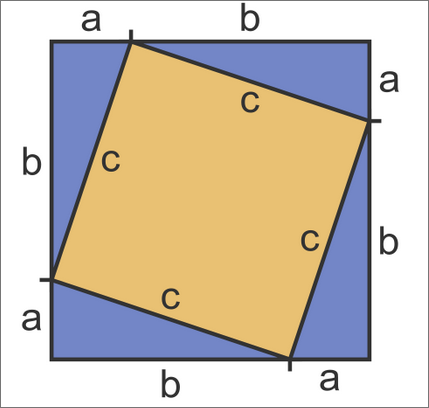
\includegraphics[width=0.2\textwidth]{resources/pythagorean-theorem-proof.png}
    \end{center}

    \vspace{0.5cm}

    L'area del quadrato esterno è data da \( (a + b)^2 \), ma anche da \( \frac{a \cdot b}{2} \cdot 4 + c^2\), da questo
    si può quindi stabilire la seguente uguaglianza:
    \[ 
       (a + b)^2 = \frac{a \cdot b}{2} \cdot 4 + c^2
    \]
    che si può semplificare
    \[ 
      a^2 + 2ab + b^2 = 2ab + c^2 
    \]
    \[ 
      a^2 + b^2 = c^2
    \]
\end{snippetproof}

\section{Somma degli angoli interni di un triangolo}

\begin{snippettheorem}{somma-angoli-interni-triangolo}{Somma degli angoli interni di un triangolo}
  La somma degli angoli interni di un triangolo è sempre 180°.
\end{snippettheorem}

\begin{snippetproof}{somma-angoli-interni-triangolo-dimostrazione}{somma-angoli-interni-triangolo}{Somma degli angoli interni di un triangolo}

  Si consideri il seguente diagramma

  \vspace{0.5cm}

  \begin{center}
      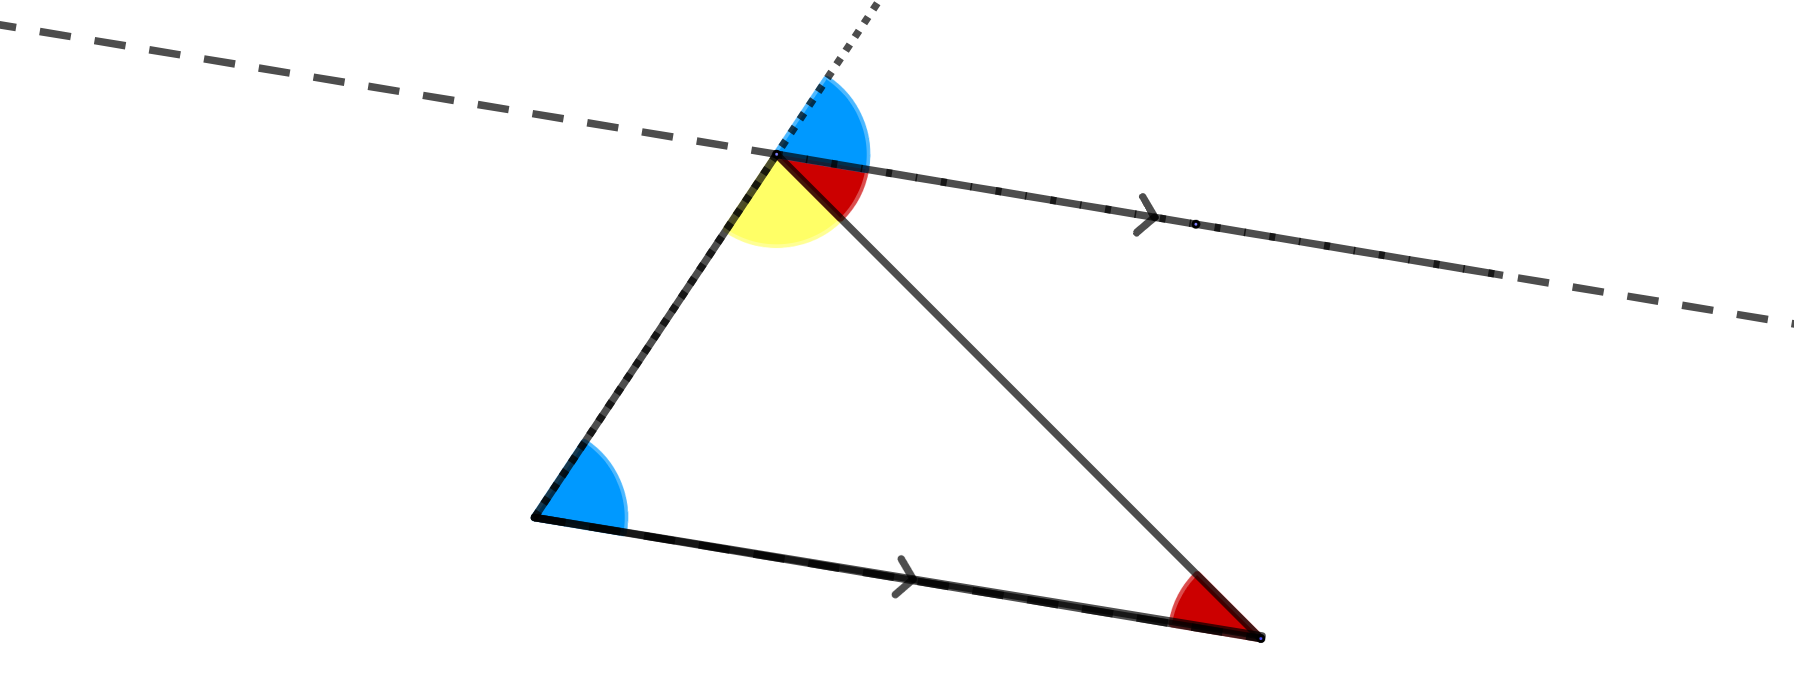
\includegraphics[width=0.5\textwidth]{resources/internal-angles-triangle.png}
  \end{center}

  \vspace{0.5cm}

  Come si può vedere, la somma data dall'angolo giallo, dall'angolo blu e dall'angolo rosso formano
  un angolo piatto, di valore 180°. Questo si può fare per qualsiasi triangolo, e il risultato sarâ
  sempre lo stesso

\end{snippetproof}

\section{Quadrato di numero dispari è dispari}

\begin{snippettheorem}{dispari-quadrato}{Quadrato di un numero dispari}
  Un qualsiasi numero dispari elevato al quadrato è ancora dispari.
\end{snippettheorem}

\begin{snippetproof}{quadrato-numero-dipari-dimostrazione}{dispari-quadrato}{Quadrato di un numero dispari}
  Come prima cosa, bisogna definire cos'è un numero dispari. Questo è dato da:
  \[
    d = 2n \pm 1 
  \]
  Elevando al quadrato questa definizione, otteniamo la seguente espressione:
  \[
    (2n \pm 1)^2
  \]
  \[ 
    4n^2 \pm 4n + 1
  \]
  \[ 
    2 \cdot (2n^2 \pm 2n) + 1
  \]
  Si può affermare che la parte \((2n^2 \pm 2n) \) è sicuramente un numero intero, e quindi lo possiamo chiamare k. 
  \[ 
    2k + 1
  \]
  Si può notare che questa forma è identica alla definizione di numero dispari data in precedenza, provando
  quindi che il quadrato di un numero dispari è ancora dispari.
\end{snippetproof}

\section{Formula radicali doppi}

\begin{snippet}{formula-radicali-doppi}
  La formula risolutiva per i radicali quadratici doppi è

  \[ 
    \sqrt{a \pm \sqrt{b}} = \sqrt{\frac{a + \sqrt{a^2 - b}}{2}} \pm \sqrt{\frac{a - \sqrt{a^2 - b}}{2}}
  \]
\end{snippet}

\end{document}
